A line is a function which is straight, and they have operations that can be performed on them. If the function is not of first order, then they can have multiple gradients.
All lines follow \(y = mx + c\), where \(m\) is the gradient, and \(c\) is the y-intercept.

\section{Characteristics of Lines}
\subsection{Gradient}
\dfn{Gradient}{The gradient of a line represents how shallow or deep it is. }

\begin{plotter}
	\addplot [
		domain=-5:5,
		samples=100,
		color=black,
	]
	{2*x};
	\addlegendentry{\(2x\)}
	\addplot [
		domain=-5:5,
		samples=100,
		color=blue,
	]
	{5*x};
	\addlegendentry{\(5x\)}
\end{plotter}

\dfn{Perpendicular Lines}{One line is perpendicular to another if \(m_a = \frac{-1}{m_b}\), ie they meet at \(90 \dg\)}

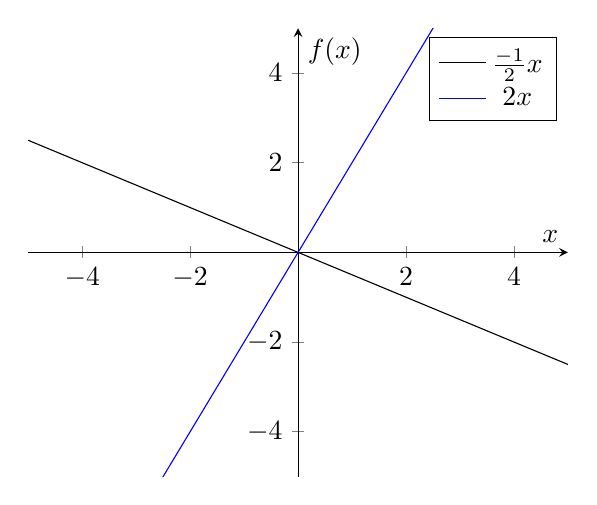
\begin{tikzpicture}
	\begin{axis}[
		axis lines = center,
		ymin=-5,ymax=5,
		xlabel = \(x\),
		ylabel = \(f(x)\),
		]
		\addplot [
		domain=-5:5,
		samples=100,
		color=black,
		]
		{-0.5*x};
		\addlegendentry{\(\frac{-1}{2}x\)}
		\addplot [
		domain=-5:5,
		samples=100,
		color=blue,
		]
		{2*x};
		\addlegendentry{\(2x\)}
	\end{axis}
\end{tikzpicture}

\subsection{Y-Intercept}

\dfn{Y Intercept}{The Y-Intercept is where the line intersects the y-axis.}
\dfn{Parallel Lines}{One line is parallel to another if the gradients are identical, but the y-intercepts are different}
\begin{plotter}
	\addplot [
		domain=-2:2,
		samples=100,
		color=black,
	]
	{x+2};
	\addlegendentry{\(x+1\)}
	\addplot [
		domain=-2:2,
		samples=100,
		color=blue,
	]
	{x-4};
	\addlegendentry{\(x-3\)}
\end{plotter}

\subsection{Lines between points}
\dfn{Midpoint}{The midpoint of a line is the average between 2 points.}
\qs{Midpoint between 2 points}{
	\ex{Between \(\left( 1,4 \right) \) and \(\left( 5,1 \right) \)}{
		\begin{align*}
			&= \left( \frac{1+5}{2} , \frac{4+1}{2} \right) \\
			&= (3, 2.5)
		\end{align*}
	}
}

\dfn{Distance}{To find the distance between 2 points, use Pythagoras.}
\qs{Distance between 2 points}{
	\ex{Between \(\left( 1,4 \right) \) and \(\left( 5,1 \right) \)}{
		\begin{align*}
			c^2 &= a^2 + b^2 \\
			c &= \sqrt{a^2 + b^2} \\
			&= \sqrt{(5-1)^2 + (4-1)^2} \\
			&= \sqrt{4^2 + 3^2}
			&= 5
		\end{align*}
	}
}

\section{Solving Line Equations}
Mainly just a question of plugging in formulas and knowing the above. One other useful thing is this:
\[ y - y_1 = m(x - x_1) \]
This equation can be used to construct a line at \((x_1, y_1)\) given gradient \(m\). This can also be used to find the y intercept.
